%File: formatting-instruction.tex
\documentclass[letterpaper]{article}
\usepackage{aaai}
\usepackage{times}
\usepackage{helvet}
\usepackage{courier}
\usepackage{graphicx}
\usepackage{url}
\usepackage{algorithm}
\usepackage{algpseudocode}

\frenchspacing
\setlength{\pdfpagewidth}{8.5in}
\setlength{\pdfpageheight}{11in}
\pdfinfo{
/Title (Implementation of RL Algorithms in OpenAI Gym)
/Author (Douglas Trajano, Sirleno Vidaletti)}
\setcounter{secnumdepth}{0}  

 \begin{document}

\title{Playing Flappy Bird with Reinforcement Learning}
\author{Douglas Trajano\\
Pontifical Catholic University of Rio Grande do Sul - PUCRS\\
School of Technology. Porto Alegre, Brazil\\
douglas.trajano@edu.pucrs.br
}
\maketitle
\begin{abstract}
\begin{quote}
Flappy Bird is an electronic game created in 2013. The objective in the game is to earn as many points as possible by controlling a bird, without letting it crash into the pipes. The Flappy Bird environment uses OpenAI Gym API. In this work, we will implement reinforcement learning algorithms such as Deep Q-Network (DQN) and Proximal Policy Gradient (PPO) that will be used to train the agent to play the game.
\end{quote}
\end{abstract}

\section{Introduction}

The Flappy Bird was released in May 2013, but it received a sudden rise in popularity in early 2014 becoming a viral hit.

The game was developed by Vietnamese programmer Dong Nguyen. It has simple gameplay, the player controls a bird, attempting to fly between green pipes without hitting them. The Flappy Bird received poor reviews from some critics, who criticized its high level of difficulty and alleged plagiarism in graphics and game mechanics, while other reviewers found it addictive.

Flappy Bird was removed from both the App Store and Google Play by its creator on February 10, 2014. He claims that he felt guilt over what he considered to be its addictive nature and overuse.

\begin{figure}[ht]
    \centering
    
\includegraphics[width=8cm]{images/flappy-bird.jpeg}
    \caption{Flappy Bird Game}
    \label{fig:flappy-bird-game}
\end{figure}

Learning to control agents directly from high-dimensional sensory inputs like vision and speech is
one of the long-standing challenges of reinforcement learning (RL). The basic idea behind many reinforcement learning algorithms is to estimate the action-value function. The goal of the agent (powered by a reinforcement learning algorithm) is to interact with the emulator by selecting actions in a way that maximizes future rewards.\cite{mnih2013playing}

We will develop some reinforcement learning algorithms that will be used to train our agents in the OpenAI Gym environment. OpenAI Gym is a toolkit for reinforcement learning research. It includes a growing collection of benchmark problems that expose a common interface.\cite{brockman2016openai}

\section{Approach}

Our technical approach consists of two parts. The first part is the definition of the environment. The environment that will be explored in this project is provided by OpenAI Gym. The second part is the reinforcement learning algorithm, which will be implemented by ourselves.

\subsection{Environment}
The Flappy Bird environment was developed by Gabriel Nogueira and is publicly available on GitHub~\footnote{\url{https://github.com/Talendar/flappy-bird-gym}}, it also can be installed using PyPI~\footnote{\url{https://pypi.org/project/flappy-bird-gym/}}. It was developed in Python and uses the OpenAI Gym API.

The state observation is composed of the horizontal distance to the next pipe and the difference between the player's y position and the next hole's y position.

Two actions are available: do nothing and jump.

\subsection{RL Algorithms}

The algorithms are responsible for learning the policy to solve the problem, it will be used to take actions in the environment. The reinforcement learning (RL) algorithms were developed in Python, we developed a base class with a random policy, it also provides the API to implement the RL algorithms. The RL algorithms are:

\subsubsection{Deep Q-Network (DQN)} combines Q-Learning with deep neural networks to let RL work for complex, high-dimensional environments, like video games, or robotics. A critical component of DQN-style algorithms is the memory buffer known as experience replay, it holds the most recent transitions collected by the policy.\cite{fedus2020revisiting}

Two different approaches of the memory buffer will be developed and tested.

\begin{itemize}
    \item \textbf{Experience Replay (ER)}: The most basic sampling strategy, it uses uniform sampling, whereby each transition in the buffer is sampled with equal probability.\cite{fedus2020revisiting}
    \item \textbf{Prioritized Experience Replay (PER)}: Extends experience replay function by learning to replay memories where the real reward significantly diverges from the expected reward, letting the agent adjust itself in response to developing incorrect assumptions.\cite{schaul2015prioritized}
\end{itemize}

\subsubsection{Proximal Policy Optimization (PPO)} is a policy gradient method that trains a stochastic policy in an on-policy way. Also, it utilizes the actor-critic method. The actor maps the observation to action and the critic gives an expectation of the rewards of the agent for the observation given. Firstly, it collects a set of trajectories for each epoch by sampling from the latest version of the stochastic policy. Then, the rewards-to-go and the advantage estimates are computed to update the policy and fit the value function. The policy is updated via a stochastic gradient ascent optimizer, while the value function is fitted via some gradient descent algorithm. This procedure is applied for many epochs until the environment is solved. \cite{schulman2017proximal}

\section{Implementation}

% What it does, what language or system it’s written in, etc.
% Use figures or screen dumps if appropriate

We developed the reinforcement learning algorithms in Python using PyTorch and Tensorflow. The source code of this project is available on GitHub~\footnote{\url{https://github.com/DougTrajano/drl-flappy-bird}}. The code is divided into two parts:

\subsection{Trainer}

The trainer is responsible for training the agents. In the training process, the environment provides observations and the agent takes actions for each observation. The Flappy Bird environment provides a reward 1 for each time step, except when the bird crashes the ground or the pipe. 

\subsection{Agents}

The agents are responsible for choosing actions for a given observation. We developed a base agent that provides the basic functions that agents should use to interact with the environment, for example, the act function receives the observation state and returns the selected action, in the base agent, the act function provides random actions based on the number of available actions. Both algorithms that we developed extend the base agent. The DQN Agent uses the experience replay (ER) or prioritized experience replay (PER), also a neural network is used to approximate the Q-function, our implementation of DQN also has an epsilon-greedy policy to handle the trade-off between exploration and exploitation. Our PPO Agent uses a Proximal Policy Optimization (PPO), a policy gradient method that uses the actor-critic method to train the policy. PPO Agent also has a buffer that uses Generalized Advantage Estimation (GAE-Lambda). We developed DQN algorithm using TensorFlow and PPO algorithm using Pytorch.

\section{Related work}

In \cite{mnih2013playing} the researchers developed the Deep Q-Network (DQN) algorithm. In this study, the agent is trained from the screen images of Atari games and it produced results far above human results. \cite{stanford2016alp} trained DQN to play Flappy Bird, the average score for the algorithm is 3.3, and the human score is 4.25. In \cite{alp2019playing} two algorithms were trained: Deep Q-Network (DQN) and Asynchronous Advantage Actor-Critic (A3C), and the results said that the A3C resulted in much faster training because it uses its own reward function. The \cite{vu2020flapai} showed that the SARSA and Q-Learning algorithms can be used to learn the Flappy Bird game. New algorithms of policy gradient methods were introduced in \cite{schulman2017proximal}, the most relevant method is proximal policy optimization (PPO) that we will implement and test in this work.

\section{Experiments}

In this experiment, we want to see if one of the two reinforcement learning algorithms that we developed can learn to play the Flappy Bird game properly.

\subsection{Trainer hyperparameters}

The following hyperparameters are used for training all the agents.

\begin{itemize}
    \item Number of episodes (n\_episodes): 60,000
    \item Early stopping (early\_stop): 120
    \item Maximum number of time steps per episode (max\_timestep): None
\end{itemize}

\subsection{DQN Agent}

The following hyperparameters are used in the DQN agent:

\begin{itemize}
    \item Dimension of each observation (state\_size): 2
    \item Quantity of available actions (action\_size): 2
    \item Random seed (seed): 1993
    \item Hidden units in the network (nb\_hidden): (64, 64)
    \item Learning rate for the optimizer (learning\_rate): 0.0005
    \item Size of the memory (memory\_size): 100,000
    \item Prioritized replay memory (prioritized\_memory): False
    \item Size of the batch to train the network (batch\_size): 64
    \item Discount factor (gamma): 0.99
    \item Interpolation parameter for target network (tau): 0.001
    \item Small value used in the priority update (small\_eps): 0.03
    \item Number of steps before updating the target network (update\_every): 4
    \item Use epsilon-greedy action selection (epsilon\_enabled): True
    \item Starting value of epsilon, for epsilon-greedy action selection (epsilon\_start): 1.0
    \item Minimum value of epsilon (epsilon\_end): 0.01
    \item Decay rate for epsilon (epsilon\_decay): 0.99995
\end{itemize}

The training session was not stopped by the early stopping policy, and the agent was trained for 60,000 episodes. Figure 2 shows the training process of the DQN agent. We can see that in 40,000 episodes, the agent achieved the best score (116.23) of the training session, but it isn't enough to stop the training.

\begin{figure}[ht]
    \centering
    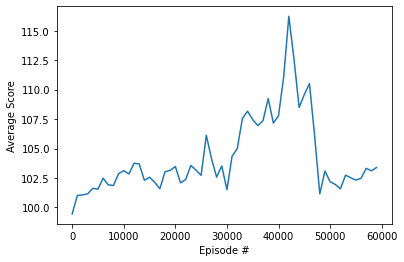
\includegraphics[width=8cm]{images/DQN_score.png}
    \caption{DQN - Average Scores by episodes}
    \label{fig:DQN-avg-scores}
\end{figure}

The DQN Agent (with 60,000 episodes) was tested in 10 trials as described in Table 1. The \textbf{Trial} column represents the number of the test, the \textbf{Env score} column represents the scores provided by the OpenAI Gym environment, and the \textbf{Skipped pipes} column represents the number of pipes skipped by the bird.

\begin{table}[h]
    \centering
    \begin{tabular}{|c||c|c|}
    \hline
    Trial & Env score & Skipped pipes \\
    \hline
    1 & 150 & 2 \\
    \hline
    2 & 114 & 1 \\
    \hline
    3 & 137 & 1 \\
    \hline
    4 & 137 & 1 \\
    \hline
    5 & 119 & 1 \\
    \hline
    6 & 121 & 1 \\
    \hline
    7 & 120 & 1 \\
    \hline
    8 & 109 & 0 \\
    \hline
    9 & 151 & 2 \\
    \hline
    10 & 114 & 1 \\
    \hline
    \end{tabular}
    \caption{DQN - Results table}
    \label{tab:dqn_table}
\end{table}

It seems that the DQN Agent learned a little bit as in the best case, the bird was able to skip only 2 pipes. The average score was 127.2, and the average number of pipes skipped was 1.1.

We developed the Prioritized Experience Replay (PER) to be used with Deep Q-Network (DQN) algorithm, but it takes a lot of time to train and it is not used in the paper.

\subsection{PPO Agent}

The following hyperparameters are used in the PPO agent:

\begin{itemize}
    \item Dimension of each observation (state\_size): 2
    \item Quantity of available actions (action\_size): 2
    \item Random seed (seed): 1993
    \item Size of the memory (memory\_size): 100,000
    \item Hidden units in the network (nb\_hidden): (64, 64)
    \item Discount factor (gamma): 0.99
    \item Lambda for GAE-Lambda (lam): 0.97
    \item KL divergence between target and current policy (target\_kl): 0.01
    \item Learning rate for the policy optimizer (policy\_lr): 0.0003
    \item Learning rate for the value function optimizer (value\_lr): 0.001
    \item Number of iterations to train the policy (train\_policy\_iters): 10
    \item Number of iterations to train the value function (train\_value\_iters): 10
    \item Clipping ratio for the policy objective (clip\_ratio): 0.2
    \item Use epsilon-greedy action selection (epsilon\_enabled): True
    \item Starting value of epsilon, for epsilon-greedy action selection (epsilon\_start): 1.0
    \item Minimum value of epsilon (epsilon\_end): 0.01
    \item Decay rate for epsilon (epsilon\_decay): 0.995
\end{itemize}

The training session was stopped when the average score of the last 100 episodes was higher than 120 in 36,029. Figure 2 shows the training process of the PPO agent. 

\begin{figure}[ht]
    \centering
    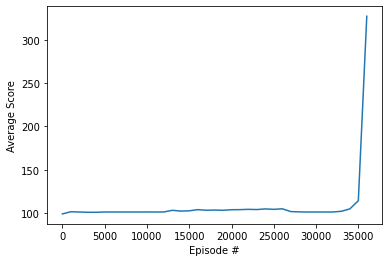
\includegraphics[width=8cm]{images/PPO_score.png}
    \caption{PPO - Average Scores by episodes}
    \label{fig:PPO-avg-scores}
\end{figure}

We can see that nearly to 35,000 episodes, the agent started to learn more quickly and finished the training achieving the stop condition (median of the last 100 scores higher than 120).

The PPO Agent (with 36,029 episodes trained) was tested in 10 trials as described in Table 2. The \textbf{Trial} column represents the number of the test, the \textbf{Env score} column represents the scores provided by the OpenAI Gym environment, and the \textbf{Skipped pipes} column represents the number of pipes skipped by the bird.

\begin{table}[h]
    \centering
    \begin{tabular}{|c||c|c|}
    \hline
    Trial & Env score & Skipped pipes \\
    \hline
    1 & 840 & 20 \\
    \hline
    2 & 692 & 16 \\
    \hline
    3 & 174 & 2 \\
    \hline
    4 & 527 & 12 \\
    \hline
    5 & 342 & 7 \\
    \hline
    6 & 506 & 11 \\
    \hline
    7 & 770 & 18 \\
    \hline
    8 & 897 & 21 \\
    \hline
    9 & 367 & 7 \\
    \hline
    10 & 1062 & 26 \\
    \hline
    \end{tabular}
    \caption{PPO - Results table}
    \label{tab:ppo_table}
\end{table}

The PPO Agent performs better than the DQN Agent, in the best case, the bird was able to skip 26 pipes. The average score was 511.5, and the average number of pipes skipped was 14.

\section{Conclusion}

Deep Reinforcement Learning (DRL) is a powerful tool for solving complex, high-dimensional environments. It can be used for video games, robotics, and many other tasks. In this paper, we developed two DRL algorithms: Deep Q-Network (DQN) and Proximal Policy Optimization (PPO). We tested the algorithms on the Flappy Bird game and showed that the PPO algorithm can learn to play the game properly. For future work, we plan to add hyperparameter tuning and other algorithms to the paper. We also want to run DQN with Prioritized Experience Replay (PER) with more time, and compare the results. We also can change the environment to use the screen of the game as the observation space.

\bibliographystyle{aaai}
\bibliography{references.bib}

\end{document}